% Shared preamble for the English summaries in this repository.
\documentclass[11pt,a4paper]{article}
\usepackage[margin=2.2cm]{geometry}
\usepackage[T1]{fontenc}
\usepackage[utf8]{inputenc}
\usepackage{lmodern}
\usepackage{amsmath,amssymb}
\usepackage{graphicx}
\usepackage{booktabs}
\usepackage{enumitem}
\usepackage[hidelinks]{hyperref}
\setlist{itemsep=2pt,topsep=4pt}
\setlength{\parindent}{0pt}
\setlength{\parskip}{5pt}
\graphicspath{{figures/}}
\newcommand{\summaryheader}[3]{%
  \begin{center}
    {\Large\bfseries #2}\\[3pt]
    {\large #1}\\[3pt]
    {\small Arshia Goshtasbi \textbullet{} MSc Electrical Engineering (Control), Iran University of Science and Technology \textbullet{} #3}
  \end{center}
  \vspace{2pt}\hrule\vspace{8pt}\par}

\begin{document}
\summaryheader{Machine Learning, Homework 2}{Supervised Regression and the Bias--Variance Trade-off}{Spring 1404 (2025)}

\textbf{Notebook} (\texttt{supervised\_regression.ipynb}). I described how scikit-learn maps the hypothesis space, risk and optimisation (HRO) view of learning onto estimators, \texttt{fit} and scoring. I listed the attributes of the Iris dataset object and the hyperparameters of \texttt{DecisionTreeRegressor}. I also wrote the empirical risk and gradient-descent update for a cubic polynomial model. On the UCI Abalone data I predicted the number of rings from the longest shell length and the whole weight with linear regression (70/30 split). The fit is $\hat y=3.54+10.33\,\text{length}+1.18\,\text{weight}$, with test MAE $1.95$ rings (Figure~\ref{fig:abalone}).

\begin{figure}[h]\centering
  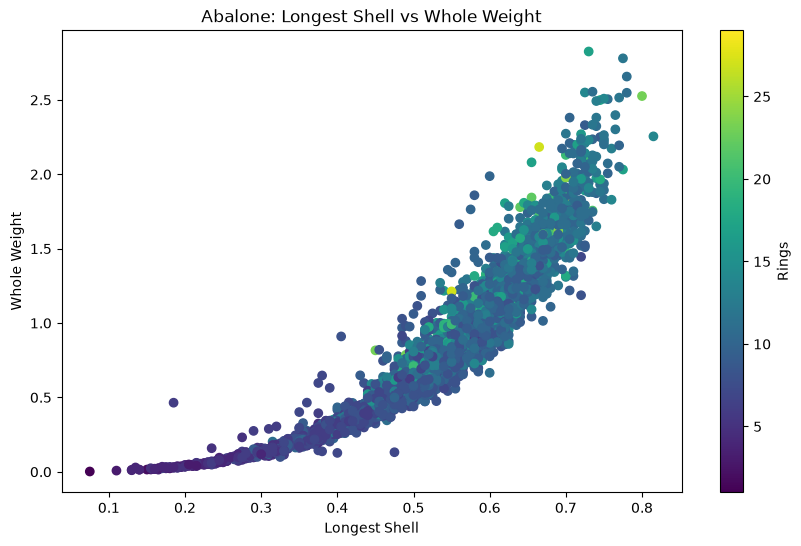
\includegraphics[width=.48\linewidth]{supervised_regression_cell21_1.png}\hfill
  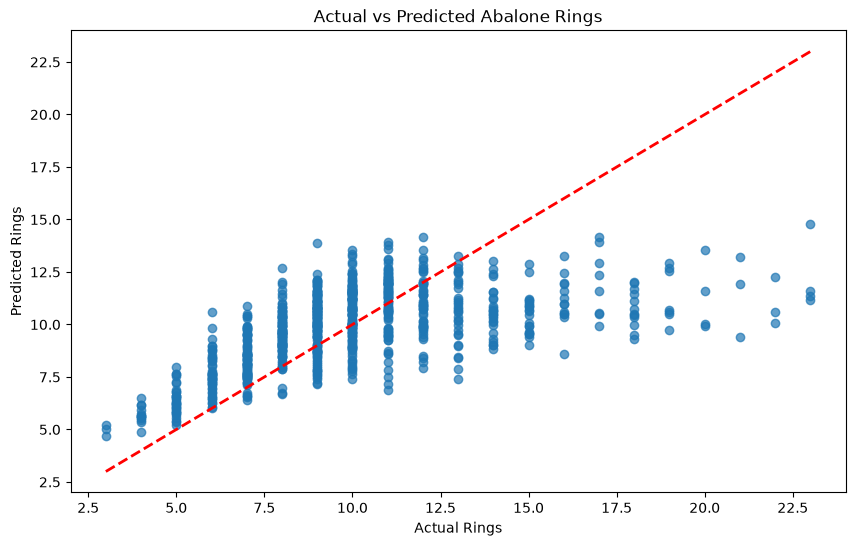
\includegraphics[width=.48\linewidth]{supervised_regression_cell26_1.png}
  \caption{Abalone: inputs coloured by rings (left), predicted vs.\ observed rings on the test set (right).}\label{fig:abalone}
\end{figure}

\textbf{Written part.}
\begin{description}
  \item[Least-squares line] (\texttt{Q2\_a.py}, \texttt{Q2\_b.py}). For the commute data, $y=18.50+0.564x$. If the teacher leaves $x$ minutes after 7:00 and must arrive by 8:40, the number of minutes early is $z=(100-a)-(1+b)x$. Setting $z=0$ gives $x\approx52$, so the latest departure is about 7:52.
  \item[Tree age from height and circumference.] With a linear model and only two inputs, the bias is high: tree type, climate and location matter and the relation is not linear. The variance is low, because the model is simple and has a million samples. The irreducible error comes from trees with the same size but different ages. The largest gain is in reducing bias, for example with more inputs and non-linear features.
  \item[Bias--variance decomposition.] I showed $\mathbb E_{D,\varepsilon}[(y-\hat y_D)^2]=\mathrm{Bias}^2+\mathrm{Var}+\sigma^2$ and explained the trade-off with $K$ in KNN (small $K$: high variance, large $K$: high bias). Bagging averages models, so it lowers variance and can raise bias slightly. Boosting fits the residuals sequentially, so it lowers bias and can raise variance.
  \item[Ridge regression as MAP.] With prior $w\sim\mathcal N(0,\alpha^2I)$ and Gaussian noise of variance $\sigma^2$, the MAP estimate equals the ridge solution with $\lambda=\sigma^2/\alpha^2$.
\end{description}
\end{document}
